\documentclass{article}

% Required packages
\usepackage{graphicx}
\usepackage{array}
\usepackage{geometry}
\usepackage{caption}
\usepackage{amsmath,amssymb}  % Added for mathematical symbols
\DeclareMathOperator*{\argmax}{argmax}
\usepackage{listings}
\usepackage{caption}
\usepackage{url}  % For URLs in bibliography

% Set page margins
\geometry{margin=1in}

% Title and author information
\title{\Large\textbf{Code Companion: Using ML to Detect Vulnerabilities in Code}}
\date{}  % Remove date

\begin{document}

% Title page
\begin{titlepage}
\begin{center}
\vspace*{2cm}
{\huge\textbf{Code Companion: Using ML to Detect Vulnerabilities in Code}\par}
\vspace{2cm}

% Authors table
\begin{tabular*}{\textwidth}{@{\extracolsep{\fill}} *{4}{c}}
    \textbf{Andrew Bevington} & \textbf{Sara Madani} & \textbf{Bryan O'Keefe} & \textbf{Alex Velsmid} \\[0.0cm]
    Computer Science & Math & Computer Science & Computer Science \\[0.0cm]
    Boston College & Bocconi University & Boston College & Boston College \\[0.0cm]
    Class of 2025 & Class of 2025 & Class of 2026 & Class of 2026 \\
\end{tabular*}

\vfill
\today
\end{center}
\end{titlepage}

\section*{Abstract}
A big problem for every software engineer and tech company is ensuring their applications are
secure. Without proper security, vulnerabilities in code can allow for hackers to gain
unauthorized access to user data and private source code. Exploits in code can negatively
affect consumers and products, which is a detrimental to companies. In the past, thousands
of lines of code would have to be manually reviewed by professionals to find and remove these
vulnerabilities. The goal of this project is to create and compare multiple machine learning algorithms that
automate the process by taking in a function written in C and running a binary classification
model on the function to label it as vulnerable or non-vulnerable. This would alleviate the pain
of manual review, and help programmers create more secure programs.

\section{Introduction}
With the rapidly increasing pace of software development as a result of modern tools like generative AI,
the need to ensure code security is becoming increasingly more valuable. According to IBM's Cost of a
Data Breach Report 2024, the average global cost of a data breach is \$4.88 million, a 10\% increase from
2023 \cite{ibm2024cost}. This highlights the critical importance of cybersecurity as more and more aspects of modern life become
digitized and connected. Therefore, cybersecurity is important in modern society as unauthorized access to
private records and data can have severe effects. In an effort to increase cybersecurity and code review
efficiency, our goal is to create and compare multiple machine learning models to accurately detect flaws in code. In order to
do so, the model would take code files as input and output a binary digit -- 0 signifying safe and 1 signifying vulnerable. Currently, there are multiple issues present with adapting a machine
learning model to cyber security efforts. These issues are noted in \cite{Arp2024}, that discusses how many top-tier security papers
from the past decade that rely on machine learning concepts exhibit three main common issues. These problems include inappropriate threat
models — where the assumed threats are not reflective of actual security risks – adversarial vulnerabilities
– where malicious inputs can deceive machine learning models – and sampling bias – when training data does
not accurately represent real-world data. In model training, the third issue of sampling bias greatly impacted the performance
of the model in a negative way if ignored and positively if considered and fixes. Before developing a model, data will be taken 
from multiple databases in order to obtain training data which is formatted and filtered to avoid duplications and inconsistencies
in syntax and layout. After collecting the data we aim to traverse through multiple experiments. Starting with the OpenAI API as
a baseline we diversify to a basic linear model used to create an Adaboost style gradient boosting network, then a GNN, and end with a transformer.

\section{Data}

\section*{Models}

\section{ChatGPT}
As a baseline we decided to explore ChatGPT 4o-mini. We approached this by first converting the data which we had from the large PrimeVul database into a more refined and focused dataset with the information that we needed and nothing more. For this, we had to implement a web scraper in order to pull the ground truth CVSS scores from the NVD website for each of the entries. After that process, we developed a script that sent a uniform vulnerability analysis query to the ChatGPT API for each function in the dataset, in order to ensure consistency across all evaluations thanks to the fixed text provided.
The prompt included a description of the setting, framing the model as a Senior Software Engineer and setting the objective at identifying vulnerabilities in the code functions. The model was then asked to return only a binary output (without explanation), which needed to be 1 if a vulnerability was present and 0 otherwise. At the end of this automatized procedure, the code saved the functions matched to their predicted label in a new file.
The initial version of the request was really detailed, explaining which scoring guidelines to refer to in evaluating the functions (CVSS 3.x), but, comparing the model’s predictions with the actual vulnerability evaluation, the accuracy registered was really low (almost 40\%). Subsequently, simplifying the prompt and making it shorter helped us improve the performance of the model, resulting in a 49.5\% success rate.
We’re actually not the first ones to attempt using large language models for vulnerability assessment. Recently (2023), some researchers from Nanyang Technological University and University of Melbourne conducted a study aimed to check whether ChatGPT is able to substitute software engineers with this kind of tasks. They divided their analysis into four different sections, changing the prompt at every step: vulnerability prediction, classification, severity estimation and repair. Our approach differs mainly in the task being framed as binary, but we can see that more or less the performances are equivalent. Indeed, their model, considering a mean of the four tasks, registered an accuracy of 45\%, so slightly less than what we obtained.


\section{Rule-Based Static Analysis for Vulnerability Detection}

In this section, we examine a rule-based static analysis system for identifying security vulnerabilities in C/C++ code. Unlike machine learning approaches that require extensive training data, this detector employs pattern matching and heuristic rules to detect common security issues. The system processes source code by tokenizing and extracting identifiers, with specialized modules targeting distinct vulnerability classes including buffer overflows, memory management issues, format string vulnerabilities, integer-related problems, and race conditions. We looked at this approach to serve as a benchmark for what could be done without the use of machine learning and see if a deterministic approach is viable for dependable vulnerability detection.

\subsection{Risk Assessment Framework}

Our implementation utilizes a risk assessment framework that assigns weights to different vulnerability categories and applies multipliers to calculate an overall risk score for each function. This approach allows for prioritization of findings rather than simple binary classification, with things like buffer overflows and array bounds violations receiving higher weights than race conditions or integer overflows. The final vulnerability determination combines the calculated risk score with the ranking to classify code as either ``Vulnerable'' or ``Safe,'' with an associated confidence rating.

Let us denote the risk score for a code snippet $c$ as:

\begin{equation}
    R(c) = \sum_{i=1}^{n} w_i \cdot I_i(c) \cdot M_i(c)
\end{equation}

where:
\begin{itemize}
    \item $w_i$ is the weight assigned to vulnerability category $i$
    \item $I_i(c)$ is the indicator function that equals 1 if vulnerability pattern $i$ is detected in code $c$, and 0 otherwise
    \item $M_i(c)$ is a multiplier based on the severity and context of the detected vulnerability pattern
    \item $n$ is the total number of vulnerability patterns examined
\end{itemize}

The classification decision is then made based on a threshold $\theta$:

\begin{equation}
    \text{Classification}(c) = 
    \begin{cases}
        \text{``Vulnerable''}, & \text{if } R(c) \geq \theta \\
        \text{``Safe''}, & \text{otherwise}
    \end{cases}
\end{equation}

\subsection{Evaluation Methodology}

We evaluated the detector on a comprehensive dataset comprising 11,947 code samples spanning multiple Common Weakness Enumeration (CWE) categories. The evaluation metrics include:

\begin{align}
    \text{Accuracy} &= \frac{TP + TN}{TP + TN + FP + FN} \\
    \text{Precision} &= \frac{TP}{TP + FP} \\
    \text{Recall} &= \frac{TP}{TP + FN} \\
    \text{F1 Score} &= 2 \cdot \frac{\text{Precision} \cdot \text{Recall}}{\text{Precision} + \text{Recall}}
\end{align}

where $TP$, $TN$, $FP$, and $FN$ represent true positives, true negatives, false positives, and false negatives, respectively.

\subsection{Performance Results}

The system achieved an accuracy of 72.21\%, with precision of 40.79\%, recall of 24.67\%, and an F1 score of 30.75\%. Table~\ref{tab:rule_based_results} summarizes the confusion matrix for our evaluation.

\begin{table}[ht]
\centering
\begin{tabular}{lcc}
\hline
& \textbf{Predicted Vulnerable} & \textbf{Predicted Safe} \\
\hline
\textbf{Actually Vulnerable} & True Positives: 737 & False Negatives: 2,250 \\
\textbf{Actually Safe} & False Positives: 1,070 & True Negatives: 7,890 \\
\hline
\end{tabular}
\caption{Confusion matrix for the rule-based vulnerability detector}
\label{tab:rule_based_results}
\end{table}

These results indicate that while the system can reliably identify safe code (high true negative rate), it struggles more with comprehensive vulnerability detection (lower recall) and generates a significant number of false alarms (lower precision).

\subsection{Performance by Vulnerability Type}

Analysis of performance across specific CWE categories reveals considerable variation in detection capabilities, as shown in Table~\ref{tab:cwe_performance}.

\begin{table}[ht]
\centering
\begin{tabular}{lccc}
\hline
\textbf{Vulnerability Type} & \textbf{CWE} & \textbf{Sample Size} & \textbf{Detection Rate} \\
\hline
Missing Authentication & CWE-255 & Limited & 100.00\% \\
Reference Time Comparison & CWE-273 & Limited & 100.00\% \\
Access Control Problems & CWE-639 & Limited & 100.00\% \\
Resource Management Errors & CWE-772 & Moderate & 31.71\% \\
Command Injection & CWE-78 & Moderate & 30.43\% \\
Denial of Service & CWE-400 & Moderate & 14.63\% \\
Memory Corruption & CWE-119 & 757 & 16.25\% \\
Use-After-Free & CWE-416 & 357 & 9.24\% \\
Improper Input Validation & CWE-20 & 568 & 11.62\% \\
\hline
\end{tabular}
\caption{Detection rates by Common Weakness Enumeration (CWE) category}
\label{tab:cwe_performance}
\end{table}

The detector performed relatively well on certain vulnerability types, including missing authentication (CWE-255), reference time comparison issues (CWE-273), and access control problems (CWE-639), all achieving 100\% detection rates, albeit on limited samples. More substantively, the detector showed moderate performance on issues like resource management errors (CWE-772) with 31.71\% detection rate, command injection vulnerabilities (CWE-78) with 30.43\% detection, and denial of service vulnerabilities (CWE-400) with a 14.63\% detection rate.

However, the system demonstrated notable weaknesses in detecting certain critical vulnerability categories. For memory corruption vulnerabilities (CWE-119), which represented a significant portion of the dataset with 757 samples, the detection rate was only 16.25\%. Similarly, for use-after-free vulnerabilities (CWE-416) with 357 samples, the detection rate was just 9.24\%. The detector also struggled with improper input validation (CWE-20), achieving only an 11.62\% detection rate across 568 samples.

\subsection{Advantages and Limitations}

The rule-based approach demonstrates several advantages, including its ability to identify multiple vulnerability classes without training data. However, the relatively low precision and recall metrics highlight the limitations inherent to pattern-based detection. The reliance on regular expressions for code parsing inhibits the ability to comprehensively reason about the code in relation to the setting around it. These limitations likely contributed to both the high false negative rate and moderate false positive rate observed in our evaluation.

\subsection{Implications and Applications}
In the context of comprehensive security analysis, this rule-based detector provides a valuable baseline approach with advantages in interpretability, efficiency, and independence from labeled training data. While it does not match the detection capabilities of state-of-the-art techniques, particularly for complex vulnerability categories, it offers an accessible entry point for vulnerability detection that can be readily integrated into development workflows and serves as a foundation for more sophisticated analysis approaches.

The significant variation in detection rates across different vulnerability categories suggests that a hybrid approach combining rule-based detection with more advanced techniques might be beneficial. In particular, the strong performance on certain well-defined vulnerability patterns indicates that rule-based components could complement learning-based approaches by providing targeted detection for specific vulnerability classes.

\section{Machine Learning-Based Vulnerability Detection: $\newline$Model Structure and Performance Analysis}

In this section, we present a hybrid approach to vulnerability detection that combines statistical machine learning techniques with rule-based feature extraction. Unlike purely rule-based approaches described in Section \textbf{X.X}, our model leverages both pattern-based features and learned representations to identify potential security vulnerabilities in C/C++ code.

\subsection{Model Architecture}

Our vulnerability detection system, \texttt{BalancedVulnDetector}, employs a two-pronged feature extraction approach followed by a classification model:

\begin{enumerate}
    \item \textbf{Text-based feature extraction}: We utilize a \texttt{HashingVectorizer} to transform code snippets into a high-dimensional sparse representation, capturing n-gram patterns within the code:
    
    \begin{equation}
        \mathbf{X}_{\text{text}} = \phi_{\text{text}}(c) \in \mathbb{R}^{n \times d_{\text{text}}}
    \end{equation}
    
    where $c$ represents a code snippet, $\phi_{\text{text}}$ is the hashing vectorizer transformation, and $d_{\text{text}}$ is the dimensionality of the text features (set to 1000 in our code).
    
    \item \textbf{Vulnerability-specific feature extraction}: We implement a custom feature extractor (\texttt{VulnFeatureExtractor}) that identifies both vulnerability patterns and safety checks using regular expressions:
    
    \begin{equation}
        \mathbf{X}_{\text{code}} = \phi_{\text{code}}(c) \in \mathbb{R}^{n \times d_{\text{code}}}
    \end{equation}
    
    where $\phi_{\text{code}}$ represents the vulnerability-specific feature extraction function.
\end{enumerate}

The combined feature representation is given by:

\begin{equation}
    \mathbf{X}_{\text{combined}} = [\mathbf{X}_{\text{text}} \; \mathbf{X}_{\text{code}}] \in \mathbb{R}^{n \times (d_{\text{text}} + d_{\text{code}})}
\end{equation}

For classification, we employ a Random Forest classifier with calibrated class weights to handle class imbalance. The probability of a code snippet being vulnerable is modeled as:

\begin{equation}
    P(y=1|\mathbf{X}_{\text{combined}}) = f_{\text{RF}}(\mathbf{X}_{\text{combined}}; \theta)
\end{equation}

where $f_{\text{RF}}$ is the Random Forest classifier and $\theta$ represents the model parameters.

\subsection{Class Imbalance Handling}

To address the prevalent class imbalance in vulnerability datasets, we employ a dynamic weighting strategy:

\begin{equation}
    w_i = 
    \begin{cases}
        1.0, & \text{if } i = 0 \text{ (non-vulnerable)} \\
        \frac{N}{2 \times N_{\text{vuln}}}, & \text{if } i = 1 \text{ (vulnerable)}
    \end{cases}
\end{equation}

where $N$ is the total number of samples and $N_{\text{vuln}}$ is the number of vulnerable samples. This approach ensures that vulnerable samples receive a controllably higher importance during training, decreasing the bias towards the majority class.

\subsection{Threshold Optimization}

We also optimized the classification threshold to balance recall and the review burden (the amount of code that is flagged as vulnerable and therefore in need of review):

\begin{equation}
    \text{score}(\tau) = 0.7 \times \text{recall}(\tau) - 0.3 \times \text{review burden}(\tau)
\end{equation}

with an adjustment factor for recall below a critical threshold:

\begin{equation}
    \text{adjusted score}(\tau) = 
    \begin{cases}
        \text{score}(\tau), & \text{if recall}(\tau) \geq 0.8 \\
        \text{score}(\tau) \times \frac{\text{recall}(\tau)}{0.8}, & \text{otherwise}
    \end{cases}
\end{equation}

where $\tau$ represents a possible threshold. The review burden is defined as the proportion of samples classified as vulnerable:

\begin{equation}
    \text{review burden}(\tau) = \frac{TP(\tau) + FP(\tau)}{N}
\end{equation}

The optimal threshold $\tau^*$ is determined by:

\begin{equation}
    \tau^* = \argmax_{\tau \in [0.3, 0.9]} \text{adjusted score}(\tau)
\end{equation}

\subsection{Detection Analysis}

Beyond binary classification, our system performs rule-based analysis to identify specific vulnerability types. For each code snippet, we apply a series of pattern-matching rules and return structured results:

\begin{equation}
    \text{analyze}(c) = \{\text{is\_vulnerable}, \text{probability}, \text{issues}\}
\end{equation}

where \texttt{issues} is a list of detected vulnerability types and descriptions.

\subsection{Experimental Results}

We evaluated our model on a comprehensive dataset of C/C++ code samples. The performance metrics are as follows:

\begin{table}[ht]
\centering
\begin{tabular}{lr}
\hline
\textbf{Metric} & \textbf{Value} \\
\hline
Accuracy & 0.5710 \\
Precision & 0.3498 \\
Recall & 0.8336 \\
F1 Score & 0.4928 \\
False Positive Rate & 0.5165 \\
Review Burden & 59.6\% \\
\hline
\end{tabular}
\caption{Performance metrics of the machine learning-based vulnerability detector}
\label{tab:ml_detector_performance}
\end{table}

\pagebreak

The confusion matrix reveals the distribution of predictions as shown in Table~\ref{tab:confusion_matrix}.

\begin{table}[ht]
\centering
\begin{tabular}{lcc}
\hline
& \textbf{Predicted Vulnerable} & \textbf{Predicted Safe} \\
\hline
\textbf{Actually Vulnerable} & True Positives: 2,490 & False Negatives: 497 \\
\textbf{Actually Safe} & False Positives: 4,628 & True Negatives: 4,332 \\
\hline
\end{tabular}
\caption{Confusion matrix for the vulnerability detection model}
\label{tab:confusion_matrix}
\end{table}

These results indicate that our model achieves high recall (83.36\%), effectively identifying most vulnerable code snippets. However, the precision is relatively low (34.98\%), resulting in a significant number of false positives.

The vulnerability type analysis shows that our model is particularly effective at detecting general vulnerabilities (83.4\% recall for the ``Other'' category). However, the model's performance may vary across specific vulnerability types.

\subsection{Comparative Analysis}

Comparing our machine learning approach with the rule-based system described in Section \textbf{X.X}, we observe significant differences in detection capabilities, as shown in Table~\ref{tab:comparative_analysis}.

\begin{table}[ht]
\centering
\begin{tabular}{lcc}
\hline
\textbf{Metric} & \textbf{Rule-Based System} & \textbf{ML-Based System} \\
\hline
Accuracy & 72.21\% & 57.10\% \\
Precision & 40.79\% & 34.98\% \\
Recall & 24.67\% & 83.36\% \\
F1 Score & 30.75\% & 49.28\% \\
\hline
\end{tabular}
\caption{Comparative analysis of rule-based and machine learning-based approaches}
\label{tab:comparative_analysis}
\end{table}

This comparison highlights a fundamental trade-off: the rule-based system achieves higher precision and accuracy but misses many vulnerabilities (low recall), while our machine learning approach prioritizes vulnerability detection (high recall) at the cost of more false positives (lower precision).

The substantial improvement in recall (from 24.67\% to 83.36\%) suggests that our hybrid approach effectively captures vulnerability patterns that rule-based systems miss. However, the increased review burden (59.6\%) may present practical challenges for integration into development workflows.

\subsection{Limitations and Future Work}

Despite the promising recall, our model faces several limitations:

\begin{enumerate}
    \item The relatively high false positive rate (51.65\%) indicates room for improvement in distinguishing between vulnerable and safe code.
    
    \item The current feature extraction approach may not fully capture semantic relationships and data flow information that are crucial for certain vulnerability classes.
    
    \item The model's performance varies across different vulnerability types, suggesting that specialized models or ensemble approaches might be beneficial.
\end{enumerate}

Future work should explore deeper code representations, potentially incorporating abstract syntax trees or program dependency graphs, to improve precision while maintaining high recall. Additionally, incremental learning strategies could help adapt the model to evolving vulnerability patterns over time.

\section{Graph Neural Network}

\subsection{Problem Formulation}
To detect code vulnerabilities at the function level, many researchers have leveraged the use of Graph Neural Networks (GNNs) \cite{ample, devign}. We frame the task of identifying vulnerable functions as a binary classification problem. Let a sample of data be defined as follows: 
\((c_i, y_i) \in D\), \( i \in \{1, \ldots, n\} \) where $n$ is the number of entries in the dataset, D is the dataset, $c_i$ is the code sample for entry $i$, and $y_i \in \{0, 1\}$ is the vulnerability label for that sample. $c_i$ is then encoded as a graph represented as follows: $G(V, E)$, where $V$ is the set of vertices and $E$ the set of edges (in the form of an edge index array). Each graph also has a corresponding node feature matrix $X$, and an edge-attribute matrix $A$. Each node, $v_i \in V$, typically corresponds to a program-element such as a variable or function call. Each edge $e_i \in E$ captures semantic information such as control flow or data. The goal of this GNN is to learn a mapping from $G$ to $Y$, $f: G \to Y$, to predict whether a function contains a vulnerability or not. The function $f$ can be learned by minimizing the following function:
\[min\sum_{i=1}^{n}L(f(G_i(V, E)), y_i | c_i) + \lambda \sum_j^m||W_j||^2] \]
where $L(\cdot)$ is the focal loss function \eqref{eq:focal-loss} \cite{focalloss} , $m$ is the number of learnable weight matrices, and $W_j$ represents the j-th weight matrix.
\begin{equation}
\mathcal{L}_{\text{focal}} = -\alpha_t (1 - p_t)^\gamma \log(p_t)
\label{eq:focal-loss}
\end{equation}

Here, $p_t$ is the predicted probability for the true class, and $\alpha_t$ and $\gamma$ are tunable hyperparameters for class weighting and focusing, respectively.


\subsection{Data Processing}
\subsubsection{Dataset Preparation}
A majority of code vulnerabilities contain a large data imbalance between vulnerable and safe functions, with vulnerable entries being in the minority. To address this, we combined \textit{PrimeVul} \cite{primevul}, \textit{BigVul} \cite{bigvul}, and \textit{DiverseVul} \cite{diversevul} datasets. Dataset statistics are contained in Table \ref{tab:dataset_entries}. Duplicate entries between datasets were removed in the combined dataset. Combining these datasets will help the model generalize more effectively.
\begin{table}[h]
    \centering
    \begin{tabular}{|l|c|c|c|}
        \hline
        Dataset & Total Entries & Vulnerable Entries & Safe Entries \\
        \hline
        PrimeVul & 224,533 & 6,004 & 218,529 \\
        BigVul & 185,997 & 10,786 & 175,211 \\
        Diversevul & 330,492 & 18,945 & 311,547 \\
        Combined & 535,951 & 29,867 & 506,084 \\
        \hline
    \end{tabular}
    \caption{Number of Total, Vulnerable, and Safe Entries in Various Datasets}
    \label{tab:dataset_entries}
\end{table}

\subsubsection{Graph Embedding}
During graph generation, code is extracted from each entry in the database. The code is not standardized, and passed into graph generation as-is. An example non-vulnerable function from the PrimeVul dataset can be seen in Code Block \ref{lst:code_example}. Then, a joint graph is generated for each function, using similar strategies to the URG-J algorithm described in \cite{jointgraph}. An example graph can be seen in Figure \ref{fig:graph_example}.

\begin{figure}[htbp]
  \centering
  \begin{minipage}{0.95\linewidth}
  \renewcommand{\lstlistingname}{Code Block}
  \begin{lstlisting}[language=C++, caption={Example C++ function that checks for metadata presence.}, label={lst:code_example}]
bool findMetadata(const Metadata::Filter& filter, const int32_t val) {
   if (filter.isEmpty()) return false;
   if (filter[0] == Metadata::kAny) return true;

   return filter.indexOf(val) >= 0;
}
  \end{lstlisting}
  \end{minipage}
\end{figure}

\begin{figure}[htbp]  % 'htbp' is an option for positioning the figure (here, top, bottom, or page)
    \centering
    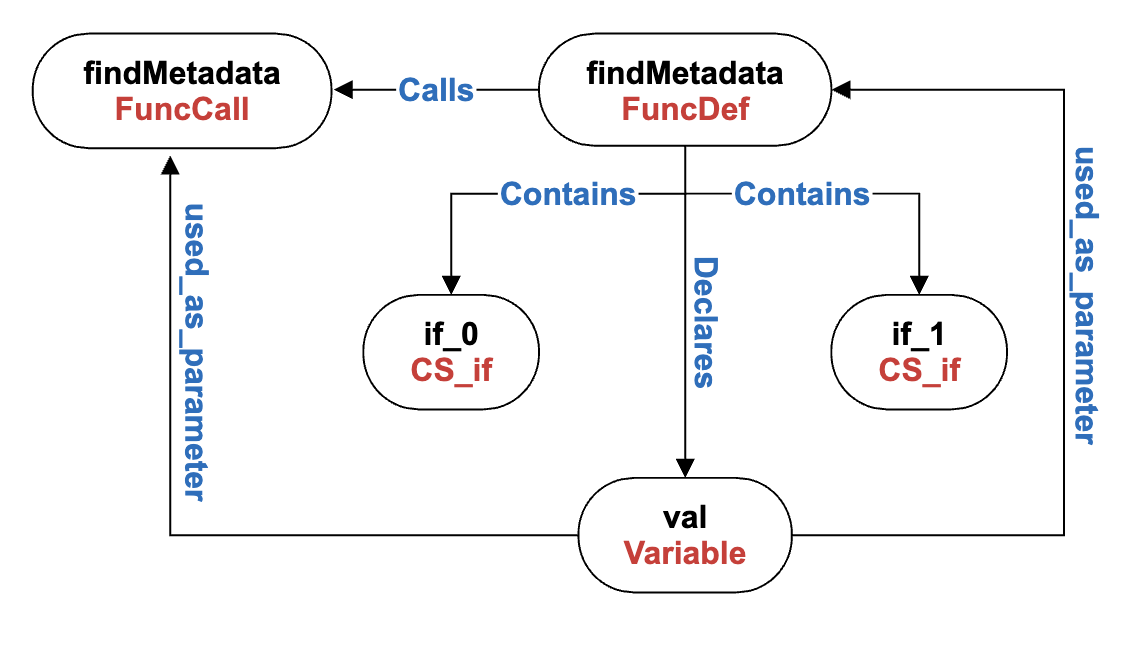
\includegraphics[width=0.6\textwidth]{graph_for_entry_9_in_db.png} 
    \caption{Graph generated from the code seen in Code Block \ref{lst:code_example}}  % The caption text
    \label{fig:graph_example}  % A label for referencing the figure in your document
\end{figure}

\subsubsection{Node Feature Matrix Generation}
Firstly, a node feature matrix, $X$, will need to be generated in order to capture node information. To capture semantic information for node identifiers (variable or function names), we utilized the popular natural-language-processing tool Word2Vec \cite{word2vec} to create vector embeddings from words. The model was trained on entire tokenized functions from the dataset. Vectors in $X$ were then generated containing: 
\begin{enumerate}
    \item A one-hot encoded vector $t_i \in {0, 1}^7$ representing the node type of node $i$. The vector contains a single 1 at the index corresponding to the node’s type (e.g., \texttt{FunctionCall}, \texttt{Variable}, etc.), and 0s elsewhere.
    \item An embedding vector $e_i \in \mathbb{R}^{100}$, computed as the average of the Word2Vec embeddings of the subtokens extracted from the node's name. If no subtokens are matched in the Word2Vec vocabulary, $e_i$ defaults to the zero vector.
\end{enumerate}
Thus, the vector $x_i \in X$ for node $v_i \in V$ is: $[t_i, e_i]^T$. 
The full node feature matrix \( X \in \mathbb{R}^{|V| \times 107} \) is defined as:

\[
X = 
\begin{bmatrix}
t_1 & t_2 & t_3 & \dots \\
e_1 & e_2 & e_3 & \dots
\end{bmatrix}
=
\begin{bmatrix}
x_1, x_2, \dots, x_{|V|}
\end{bmatrix}
\]

% Node Type Table
\begin{table}[h]
\centering
\begin{tabular}{ll}
\hline
\textbf{Node Type} & \textbf{Description} \\
\hline
\texttt{FunctionCall} & Represents a function call \\
\texttt{Variable} & A named variable in the code \\
\texttt{ControlStructure\_if} & An if-statement branch \\
\texttt{ControlStructure\_while} & A while-loop construct \\
\texttt{ControlStructure\_switch} & A switch-case block \\
\texttt{ControlStructure\_for} & A for-loop construct \\
\texttt{FunctionDefinition} & A function definition\\
\hline
\end{tabular}
\caption{Predefined node types used in graph construction.}
\label{tab:nodetypes}
\end{table}

\subsubsection{Edge Index and Edge Type Matrix Generation}
To construct the edge-related data for the GNN, we utilize two structures:

\begin{enumerate}
    \item The \textbf{edge index matrix} $E \in \mathbb{Z}^{2 \times |E|}$, which encodes the graph's edges. Each column represents a directed edge $(u, v)$, where $u$ and $v$ are node indices from the node feature matrix $X$. This is essentially an adjacency matrix compatible with PyTorch Geometric.
    \item The \textbf{edge attribute vector} $A \in \mathbb{Z}^{|E|}$, where each entry corresponds to an edge type (Table \ref{tab:edgetypes}) for the respective edge $e_i$.
\end{enumerate}
Given a graph $G = (V, E)$, we iterate over each edge $(u, v) \in E$ and extract its edge type (e.g., \texttt{calls}, \texttt{declares}, etc.). Each edge is mapped to an integer according to a pre-defined mapping. If an edge type is not recognized, it is assigned a value of $-1$ to be ignored during training. \\

Each graph $G$ is thus represented by three components: a node feature matrix $X$, the edge index matrix $E$, and the edge attribute vector $A$, which collectively define the input to the GNN model.

\begin{table}[h]
\centering
\begin{tabular}{lp{8cm}}
\hline
\textbf{Edge Type} & \textbf{Description} \\
\hline
\texttt{declares} & Indicates a declaration relationship. \\
\texttt{calls} & Represents a function call from one node to another. \\
\texttt{contains} & Denotes structural containment (e.g., a function contains a statement). \\
\texttt{used\_in\_condition} & Marks variables or expressions used in control conditions such as \texttt{if}, \texttt{while}, or \texttt{switch} statements. \\
\texttt{used\_as\_parameter} & Marks nodes that are passed as parameters to a function call. \\
\texttt{used\_in\_body} & Captures general usage of elements inside the body of a function or code block. \\
\hline
\end{tabular}
\caption{Predefined edge types used in graph construction.}
\label{tab:edgetypes}
\end{table}

\subsection{Architecture}
\subsubsection{The Convolution Layer}
Many existing graph neural network approaches to vulnerability detection have used aggregation techniques like graph convolution networks (GCNs) \cite{gcn}, graph attention networks (GATs) \cite{gat}, gated graph recurrent networks (GGRNs), and their variants. For this project, designed and tested three models, each of which using either GCNs, RGCNs, or GATs.
\paragraph{Graph Convolution Layer (GCN)}
\begin{description}
  \item[GCN \cite{gcn}:] Uses the propagation rule: 
  \[
  \mathbf{H}^{(l+1)} = \sigma\left( \tilde{\mathbf{D}}^{-\frac{1}{2}} \tilde{\mathbf{A}} \tilde{\mathbf{D}}^{-\frac{1}{2}} \mathbf{H}^{(l)} \mathbf{W}^{(l)} \right)
  \]
  where $\tilde{\mathbf{A}} = \mathbf{A} + \mathbf{I}_N$ is the adjacency matrix of the graph $G$ with added self-loops, and $\tilde{\mathbf{D}}_{ii} = \sum_j \tilde{\mathbf{A}}_{ij}$ is the corresponding degree matrix (containing the number of connected edges per node). $\mathbf{W}^{(l)}$ is the trainable weight matrix for layer $l$, and $\sigma(\cdot)$ is a nonlinear activation function like ReLU. $\mathbf{H}^{(l)}$ denotes the output node embeddings after layer $l$, with $\mathbf{H}^{(0)} = \mathbf{X}$, the initial input features.

  \item[GAT \cite{gat}:] Graph Attention Networks compute attention scores between nodes and their neighbors:
  \[
    \alpha_{ij} = \frac{\exp(\text{LeakyReLU}(\textbf{a}^T[\mathbf{W}h_i || \mathbf{W}h_j]))}{\sum_{k \in \mathcal{N}_i} \exp(\text{LeakyReLU}(\textbf{a}^T[\mathbf{W}h_i || \mathbf{W}h_k]))}
  \]
  where $\big\Vert$ represents the concatenation operation. $h_i$ represents the set of node features for node $i$. A shared linear transformation is applied to every node through the learnable weight matrix $\textbf{W}$. Additionally, a shared attention mechanism, $\textbf{a}$, is applied to every transformation, and is used to compute the importance of node $j$'s features on node $i$. $\mathcal{N}_i$ represents the set of neighbor nodes of node $i$ in the graph. $\alpha_{ij}$ represents the attention coefficient, representing the normalized importance of node $j$'s features on node $i$. Then, the result of feature aggregation, $h_i'$, is obtained through multi-head attention mechanisms as follows:
  \[
    h_{i}' = \big\Vert_{k=1}^K \sigma(\sum_{j \in \mathcal{N}_i} \alpha_{ij}^k \textbf{W}^k h_j)
  \]
  where $\alpha_{ij}^k$ are normalized attention coefficients computed at the $k^{th}$ attention mechanism and $\mathbf{W}^k$ is the linear transformation weight matrix for attention mechanism $k$.


  \item[RGCN \cite{rgcn}:] Relational Graph Convolution Networks extend GCNs to handle multiple edge types:
  \[
  \mathbf{h}_i^{(l+1)} = \sigma\left( \sum_{r \in \mathcal{R}} \sum_{j \in \mathcal{N}_i^r} \frac{1}{c_{i,r}} \mathbf{W}_r^{(l)} \mathbf{h}_j^{(l)} + \mathbf{W}_0^{(l)} \mathbf{h}_i^{(l)} \right)
  \]
  where $\mathcal{R}$ is the set of relation types, and $\mathcal{N}_i^r$ denotes the set of neighborhood indices to node $i$ of relation $r$. $\mathbf{W}_r^{(l)}$ is a learnable weight matrix specific to relation $r$. $c_{i, r}$ is a problem-specific normalization constant that can either be learned or chosen in advance. $\mathbf{W}_0^{(l)} \mathbf{h}_i^{(l)}$ is added to account for self-loop contributions.

\end{description}

\subsubsection{Model Flow}
Each of the three models follow a similar flow:
\begin{enumerate}
    \item The node features are passed through the respective graph convolution layers, followed by activation functions (ReLU) and dropout for regularization.
    \item Node features are aggregated using global mean pooling to generate graph-level embeddings.
    \item The graph-level features are concatenated with additional graph-level flags and passed through an multi-layer perceptron for the final classification.
\end{enumerate}

\subsection{Evaluation}
To assess the performance of our graph-based model, we aimed to answer the following questions: \\
\textbf{Q1: } How does our model compare to the state-of-the-art graph-based binary classification models? \\
\textbf{Q2: } Which of the convolution models provides the best performance? \\
\textbf{Q3: } What types of vulnerabilities does the model continuously fail to identify? \\
\textbf{Q4: } How does the model handle class imbalance? \\
\textbf{Q5: } What are the next steps needed to improve the performance of vulnerability detection via machine learning methods?

\subsubsection{Dataset preparation}
Many popular datasets exist for vulnerability detection; however, they all have a severe imbalance between vulnerable and non-vulnerable entries, with vulnerable entries being in the extreme minority. To that end, we chose to combine the \textit{PrimeVul} \cite{primevul}, \textit{BigVul} \cite{bigvul}, and \textit{DiverseVul} \cite{diversevul} datasets. Then, duplicate entries across datasets were removed, leaving a combined dataset with $29,867$ vulnerable entries and $506,084$ safe entries (Table \ref{tab:dataset_entries}). Safe entries were downsampled across the entire dataset. In the training dataset, vulnerable entries were randomly oversampled to achieve a 50/50 split between vulnerable and safe entries (Table \ref{tab:train-test-valid-split}). Entries in the dataset were then randomly shuffled. All of the GNN-based models were tested on the complete dataset, and the PrimeVul dataset.

\begin{table}[h]
 \centering
 \resizebox{\textwidth}{!}{ % Adjusts the table to the width of the text
 \begin{tabular}{|l|c|c|c|c|}
 \hline
 \textbf{Dataset} & \textbf{Total Entries} & \textbf{Percent Duplicates} & \textbf{Vulnerable Entries} & \textbf{Safe Entries} \\
 \hline
 \multicolumn{5}{|c|}{\textbf{Complete Dataset}} \\
 \hline
 Train & 354,258 & 44.00\% & 177,129 (50.00\%) & 177,129 (50.00\%) \\
 Test & 80,393 & 0.00\% & 4,480 (5.57\%) & 75,913 (94.43\%) \\
 Validation & 80,393 & 0.00\% & 4,480 (5.57\%) & 75,913 (94.43\%) \\
 \hline
 \multicolumn{5}{|c|}{\textbf{PrimeVul Dataset}} \\
 \hline
 Train & 8,406 & 41.67\% & 4,203 (50.00\%) & 4,203 (50.00\%) \\
 Test & 6,363 & 0.00\% & 900 (14.14\%) & 5,463 (85.86\%) \\
 Validation & 6,364 & 0.00\% & 901 (14.16\%) & 5,463 (85.84\%) \\
 \hline
 \end{tabular}
 }
 \caption{Datasets used for training, testing, and validation for Complete and PrimeVul datasets}
 \label{tab:train-test-valid-split}
\end{table}



\subsubsection{Results}
In the embedding layer, the dimension of Word2Vec for the initial node representation is 100. For the GCN, GAT, and RGCN layers, the dimension of hidden states was set to 128. Three convolution layers were used for all three convolution types. We use the Adam optimizer with a learning rate of $0.001$, and batch size of $128$. We additionally used an L2 regularization rate of $1 \times 10^{-5}$, and dropout of $0.3$ to minimize overfitting. Each model was evaluated over 25 epochs. The decision threshold was adjusted based on Youden's J statistic from the ROC curve, aiming to balance vulnerable samples and false positives. All models were tested after training using the test dataset, while during training, they were tested using the validation dataset after each epoch. See Table \ref{tab:performance-metrics} for results. 
\paragraph{GCN:} The model using the GCN convolution achieved very low precision, indicating a high number of misclassifications of safe samples as vulnerable. However, it demonstrated high recall, reflecting a strong ability to identify vulnerable samples. This is particularly valuable in vulnerability detection, where false negatives are more detrimental than false positives. Despite this, the model showed unstable validation accuracy compared to the more consistent training accuracy (Figure \ref{fig:gcn_acc}).

\paragraph{GAT:} The model using the GAT convolution achieved moderate precision, indicating a relatively low rate of misclassify safe samples as vulnerable. While its recall is also moderate, it reflects a balanced ability to identify vulnerable samples. Additionally, the model achieved precision accuracy closer to train accuracy, indicating less overfitting and better generalization (Figure \ref{fig:gat_acc}).

\paragraph{RGCN:} The model utilizing the RGCN convolution achieved a precision of 0.177—the highest among all architectures—highlighting its strong ability to minimize false positives. In terms of recall, the RGCN reached 0.639, which, while slightly lower than the values observed in GAT and GCN-based models, still reflects a strong ability to capture true positives. Additionally, the RGCN exhibited relatively stable and high validation accuracy throughout training, consistently ranging between $80$\% and $85$\% (Figure \ref{fig:rgcn_acc}).

\paragraph{Devign:} The state-of-the-art Devign model exhibited relatively high precision, indicating that it is conservative in predicting vulnerabilities and avoids misclassifying safe samples as vulnerable. However, its recall was significantly lower, meaning it misses a substantial number of true positives. Devign also demonstrated the lowest accuracy of all models at $43.6$\%.

\begin{table}[h]
    \centering
    \begin{tabular}{|l|c|c|c|c|c|}
        \hline
        \textbf{Model} & Accuracy & Precision & Recall & F1 Score & AUC \\
        \hline
        \multicolumn{6}{|c|}{\textbf{Complete Dataset}} \\
        \hline
        \textbf{GCN}  & 0.6084  & 0.1045  & 0.7960  & 0.1847  & 0.766 \\
        \textbf{GAT}  & 0.7545  & 0.1373  & 0.6444  & 0.2264  & 0.766 \\
        \textbf{RGCN} & 0.8142  & 0.1770  & 0.6393  & 0.2772  & 0.799 \\
        \textbf{Devign} & 0.4360 & 0.4470 & 0.4040 & 0.4240 & 0.453 \\
        \hline
        \multicolumn{6}{|c|}{\textbf{PrimeVul Dataset}} \\
        \hline
        \textbf{RGCN}  & 0.3929  & 0.1821  & 0.9433  & 0.3053  & 0.742 \\
        \textbf{GCN}   & 0.3442  & 0.1654  & 0.8989  & 0.2794  & 0.669 \\
        \textbf{GAT}   & 0.3539  & 0.1677  & 0.9000  & 0.2827  & 0.676 \\
        \textbf{Devign} & 0.4850 & 0.5000 & 0.4810 & 0.4900 & 0.486 \\
        \hline
    \end{tabular}
    \caption{ML Stats for Complete and PrimeVul Datasets}
    \label{tab:performance-metrics}
\end{table}

\begin{figure}[h]
    \centering
    \begin{minipage}{0.32\textwidth}
        \centering
        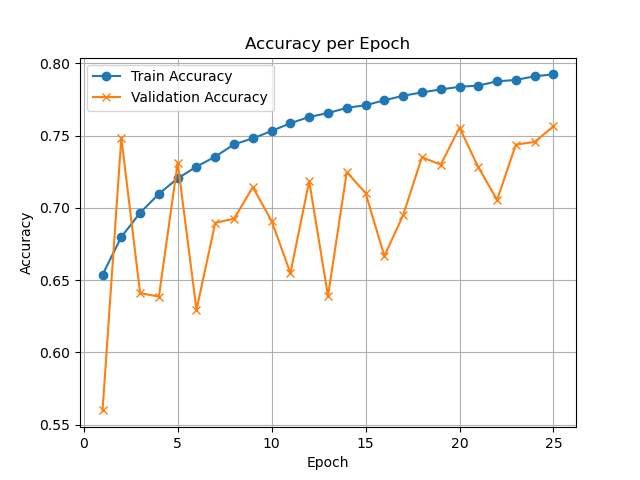
\includegraphics[width=\textwidth]{gat_acc.png}
        \caption{GAT Accuracy (Complete)}
        \label{fig:gat_acc}
    \end{minipage}
    \hfill
    \begin{minipage}{0.32\textwidth}
        \centering
        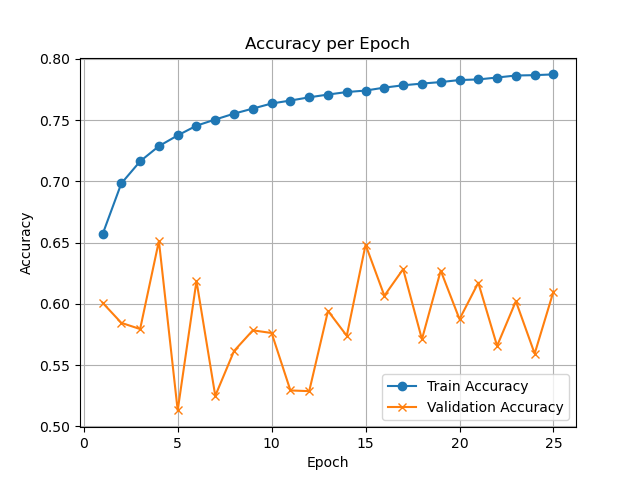
\includegraphics[width=\textwidth]{gcn_acc.png}
        \caption{GCN Accuracy (Complete)}
        \label{fig:gcn_acc}
    \end{minipage}
    \hfill
    \begin{minipage}{0.32\textwidth}
        \centering
        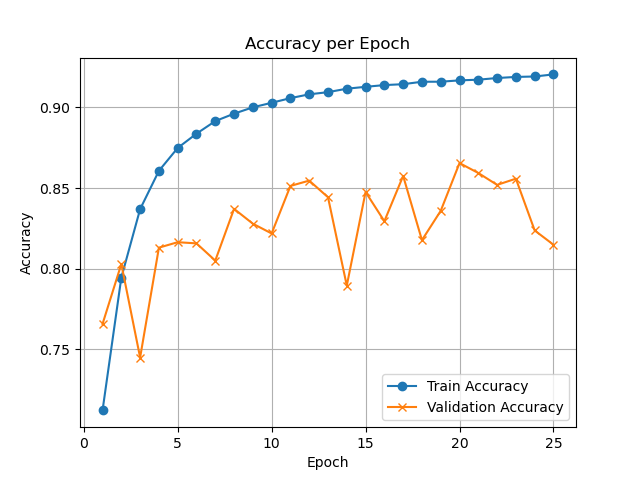
\includegraphics[width=\textwidth]{rgcn_acc.png}
        \caption{RGCN Accuracy (Complete)}
        \label{fig:rgcn_acc}
    \end{minipage}
    
    \vspace{0.5cm} % Adds a little space between rows
    
    \begin{minipage}{0.32\textwidth}
        \centering
        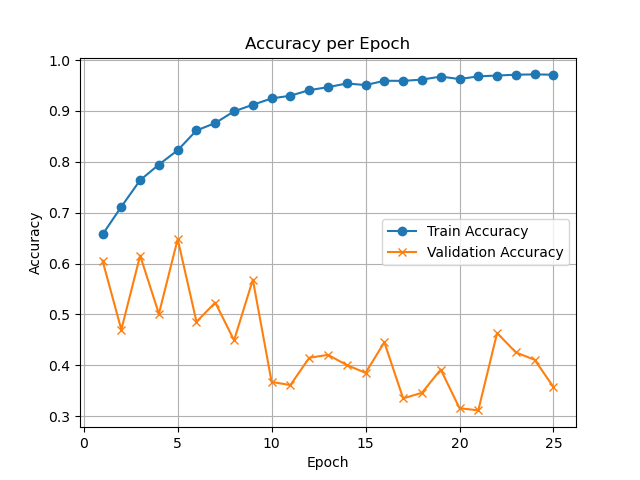
\includegraphics[width=\textwidth]{pv_gat_acc.png}
        \caption{GAT Accuracy (PrimeVul)}
        \label{fig:pv_gat_acc}
    \end{minipage}
    \hfill
    \begin{minipage}{0.32\textwidth}
        \centering
        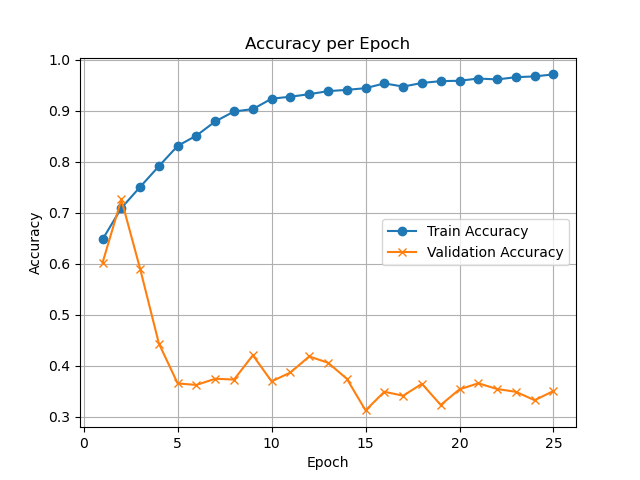
\includegraphics[width=\textwidth]{pv_gcn_acc.png}
        \caption{GCN Accuracy (PrimeVul)}
        \label{fig:pv_gcn_acc}
    \end{minipage}
    \hfill
    \begin{minipage}{0.32\textwidth}
        \centering
        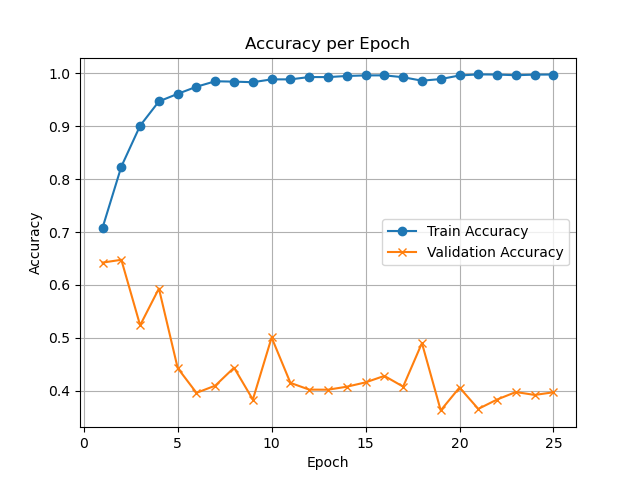
\includegraphics[width=\textwidth]{pv_rgcn_acc.png}
        \caption{RGCN Accuracy (PrimeVul)}
        \label{fig:pv_rgcn_acc}
    \end{minipage}

    \caption{Accuracy Curves for GAT, GCN, and RGCN across Complete and PrimeVul Datasets}
    \label{fig:acc_curves}
\end{figure}

\paragraph{Performance on specific vulnerabilities:}\label{sec:performance-on-vulns} Based on results from the RGCN model, the model classified the following vulnerabilities well: authentication bypass, improper initialization, and missing encryption, achieving $100$\% detection rates on all three (Table \ref{tab:vulnerabilities}). The model fails to fully identify the following vulnerabilities: resource management error, information exposure, race condition, numeric error, and inadequate access controls, only achieving between $60$-$70$\% detection on these vulnerabilities (Table \ref{tab:vulnerabilities}).

\begin{table}[h]
    \centering
    \resizebox{\textwidth}{!}{
    \begin{tabular}{|l|c|c|c|}
        \hline
        \textbf{Vulnerability Type} & \textbf{CWE} & \textbf{Sample Size} & \textbf{Detection Rate (\%)} \\ 
        \hline
        \multicolumn{4}{|c|}{\textbf{Best Performing}} \\
        \hline
        Authentication Bypass & CWE-290 & 21 & 100.00\% \\
        Improper Initialization & CWE-665 & 15 & 100.00\% \\
        Missing Encryption & CWE-311 & 52 & 100.00\% \\
        \hline
        \multicolumn{4}{|c|}{\textbf{Worst Performing}} \\
        \hline
        Resource Management Error & CWE-399 & 4218 & 63.00\% \\
        Information Exposure & CWE-200 & 4865 & 65.60\% \\
        Race Condition & CWE-362 & 2755 & 69.30\% \\
        Numeric Error & CWE-189 & 4093 & 65.30\% \\
        Inadequate Access Controls & CWE-772 & 996 & 61.00\% \\
        \hline
    \end{tabular}
}
\caption{Comparison of Best and Worst Performing Vulnerabilities}
\label{tab:vulnerabilities}
\end{table}

\subsubsection{Discussion}
The results indicate that, while Graph Neural Networks (GNNs) show potential in vulnerability detection, there remains significant room for improvement, especially when considering the low F1 scores observed across all models. The trade-offs between precision, recall, and F1 score highlight the challenges of achieving a balanced and effective model for vulnerability detection.

\paragraph{Comparison Between Datasets:} 
A notable comparison is between the performance on the Complete dataset and the PrimeVul dataset. While the models performed relatively well on the Complete dataset, achieving an accuracy of around 60-80\% for GCN, GAT, and RGCN, the performance on the PrimeVul dataset alone was much lower. Though the F1 scores are misleadingly higher (Table \ref{tab:performance-metrics}), the  accuracy is extremely low. Additionally, during training, the validation accuracy plummets, indicating the PrimeVul dataset alone does not have enough information to allow the model to generalize. Thus, all models were trained on the combined dataset.

\paragraph{Precision vs Recall}
The GCN model demonstrated high recall but very low precision, meaning that while it was able to identify many of the vulnerable samples, it frequently misclassified safe samples as vulnerable. While it is important in vulnerability detection to minimize false negatives (i.e. avoid misclassifying vulnerable code as safe), the low F1 score, precision, and accuracy indicates the model is not generalizing well on the data.

In contrast, the GAT model displayed more stable validation accuracy, suggesting that it has better generalization capabilities. The model also demonstrates higher accuracy, precision, recall, and F1, indicating the GAT convolution is better at learning vulnerability patterns from the graph. However, there is still a lot of room for improvement.

The RGCN model performed the best overall, with the highest F1 score and validation accuracy. Though it has lower recall as compared to the GAT and GCN, it demonstrates the best balance between precision and recall. Additionally, its stable and high validation accuracy indicates a better ability to generalize insights from the train data on the validation dataset. Overall, the high accuracy and F1 achieved using the RGCN convolution make it the most reliable for vulnerability detection in this study. However, its slightly lower recall compared to the GCN suggests that further improvements can be made to maximize its sensitivity to vulnerabilities.

\paragraph{Most Frequently Misclassified Vulnerabilities:} While the model is good at detecting certain vulnerabilities (Table \ref{tab:vulnerabilities}), the sample sizes for these vulnerabilities is fairly low and inconclusive. The worst performing vulnerabilities, including resource management error, information exposure, race condition, numeric error, and inadequate access controls, involve complex patterns that the model may struggle to identify. Though a detection rate of $60$-$70$\% is not ideal, it is still better than a random guess. 

\paragraph{Devign}
The state-of-the-art Devign model utilizes word embeddings (with Word2Vec) with graph-based features, similarly to our model. Devign uses Joern \cite{joern}, a pre-existing tool to generate complex code property graphs, as compared to our fairly simple graph representations. Devign also utilizes Gated Graph Recurrent Networks \cite{ggrn}, where we use GCNs, GATs, and RGCNs. Devign showed relatively high precision, meaning it is cautious in predicting vulnerabilities and avoids misclassifying safe samples as vulnerable. However, its low recall indicates that it misses a significant portion of true vulnerabilities. The model also demonstrated the lowest accuracy and AUC among all models, which indicates that Devign struggles to generalize well to the validation dataset. The combination of low recall and accuracy points to significant limitations in its ability to perform well in vulnerability detection on the current dataset.

\paragraph{Conclusion}
The low F1 scores across all architectures suggest that there is still much to be done to improve the models' performance, particularly in terms of increasing recall while maintaining precision. A possible approach to achieving this goal would be to improve graph expression of data. One popular graph generation tool is Joern \cite{joern}, which generates more complex code property graphs (CPGs). Along with this, further exploration of feature engineering could help create better code context, helping the model detect complex vulnerabilities easier. Additionally, further work will need to be done to find vulnerable samples, as the massive class imbalance in the dataset has limited the performance of the model.

Overall, when comparing our model with the state-of-the-art model Devign, it is clear we have made some improvements toward vulnerability detection. However, more work will need to be done in order to detect complex vulnerabilities more reliably.

\section{Transformer Block Overview}

Transformers are neural network architectures designed to process inputs represented as unordered sets of tokens. Each token \( x_n^{(0)} \) is a vector in \( \mathbb{R}^D \), and the full input is arranged as a matrix \( X^{(0)} \in \mathbb{R}^{D \times N} \), where \( N \) is the number of tokens and \( D \) is the feature dimension. This design allows transformers to handle diverse data types, such as text or image patches, using a unified architecture. As Turner notes, this removes the need for ``bespoke handcrafted architectures for mixing data of different modalities' \cite{turner2024introductiontransformers}. The transformer operates by applying a block of operations repeatedly to the input:

\[
X^{(m)} = \text{transformer-block}(X^{(m-1)})
\]

Each block consists of two main stages:
\begin{itemize}
  \item \textbf{Stage 1: Self-Attention across the sequence}
  \item \textbf{Stage 2: Multi-Layer Perceptron (MLP) across features}
\end{itemize}

\subsection{Stage 1: Self-Attention}

Self‐attention allows each token to incorporate information from the entire sequence by computing a weighted sum of all input representations.  Given input matrix \(X^{(m-1)}\in\mathbb{R}^{D\times N}\), we first project into queries and keys:
\[
q_n \;=\; U_q\,x_n,\qquad
k_n \;=\; U_k\,x_n,
\quad
U_q,\,U_k\in\mathbb{R}^{d_k\times D},\;n=1,\dots,N.
\]
Next, we form the raw score matrix \(W\in\mathbb{R}^{N\times N}\) with scaled dot‐products:
\[
W_{n,n'}
=\frac{q_n^{\!\top}k_{n'}}{\sqrt{d_k}}
\qquad
(n,n'=1,\dots,N).
\]
We then normalize each row of \(W\) via a softmax to obtain the attention weights:
\[
A_{n,n'}
=\mathrm{softmax}\bigl(W_{n,\ast}\bigr)_{n'}
=\frac{\exp\bigl(W_{n,n'}\bigr)}
      {\sum_{n''=1}^N\exp\bigl(W_{n,n''}\bigr)}.
\]
Finally, the output of the self‐attention layer is the weighted sum
\[
Y^{(m)}
= X^{(m-1)}\,A^{(m)},
\]
where \(A^{(m)}\) collects the weights \(A_{n,n'}\).  
This introduces the projections 
\[
q_n = U_q x_n,\quad k_n = U_k x_n,
\]
which map each input vector into a “query” and “key” space where similarity scores are computed.  In effect, self-attention re-expresses each vector as a weighted sum of all inputs: if \(A\) and \(B\) are similar (high dot-product in query/key space), then their outputs both become roughly \(A+B\), and similarly for other groups like \(C\) and \(D\).  This lets the model dynamically aggregate information from semantically related tokens.

\subsection{Multi‐Head Self‐Attention (MHSA)}

To allow the model to attend to information in different representational subspaces, multi‐head self‐attention applies \(H\) independent heads in parallel:

\[
\text{head}_h^{(m)}
= V_h \,X^{(m-1)}\,A_h^{(m)},
\qquad h=1,\dots,H,
\]
where each attention matrix is
\[
[A_h^{(m)}]_{n,n'}
=\frac{\exp\bigl((k_{h,n}^{(m)})^\top q_{h,n'}^{(m)}\bigr)}
      {\sum_{n''=1}^N\exp\bigl((k_{h,n''}^{(m)})^\top q_{h,n'}^{(m)}\bigr)},
\]
and
\[
q_{h,n}^{(m)}=U_{q,h}^{(m)}\,x_n^{(m-1)},
\quad
k_{h,n}^{(m)}=U_{k,h}^{(m)}\,x_n^{(m-1)}.
\]

Rather than summing the heads, we **concatenate** their outputs and apply a final linear projection \(W^O\in\mathbb{R}^{D\times (H\,D)}\):

\[
Y^{(m)}
= W^O \;\bigl[\text{head}_1^{(m)} \,\|\, \text{head}_2^{(m)} \,\|\, \cdots \,\|\, \text{head}_H^{(m)}\bigr],
\]
where \(\|\) denotes concatenation along the feature dimension.  


\subsection{Stage 2: MLP Across Features}

After self-attention, each token's vector is refined using a non-linear transformation, applied independently across tokens:

\[
x_n^{(m)} = \text{MLP}(y_n^{(m)})
\]

This operation is akin to the update step in Graph Neural Networks. \cite{turner2024introductiontransformers}

\subsection{Stabilization: Residual Connections and Normalisation}

Each sub-layer is wrapped with a residual connection:

\[
x^{(m)} = x^{(m-1)} + \text{residual}(x^{(m-1)})
\]

and uses \textbf{Layer Normalisation} (referred to in the paper as ``TokenNorm''):

\[
\text{LayerNorm}(x_{d,n}) = \frac{x_{d,n} - \mu_n}{\sqrt{\sigma_n^2}} \gamma_d + \beta_d
\]

where

\[
\mu_n = \frac{1}{D} \sum_{d=1}^D x_{d,n}, \quad \sigma_n^2 = \frac{1}{D} \sum_{d=1}^D (x_{d,n} - \mu_n)^2
\]

and \( \gamma_d, \beta_d \) are learned scale and shift parameters.

\subsection{Positional Encoding}

Because transformers are permutation-invariant, they require additional information to capture token order. This is done by adding or concatenating a positional embedding to each token:

\[
x_n^{(0)} = W p_n + e_n
\]

where \( p_n \) is the input patch or token, \( W \) is the patch embedding matrix, and \( e_n \) is the position embedding. \cite{turner2024introductiontransformers}

\subsection{Conclusion}

The transformer architecture consists of stacked transformer blocks, each combining multi-head self-attention and MLP layers, along with residual connections and layer normalization. By processing sequences in this way, transformers can model complex dependencies across tokens and have become a foundational tool in modern machine learning.

\section{CodeT5}
CodeT5 is a T5 model transformer model created by the Saleforce Research group. This model was created to be more apt at handling code and thus improve software development. The separating factor from CodeT5 and other transformer models like BERT and GPT is that it implements an encoder-decoder architecture which allows for better code understanding and generation. BERT is an encoder-only model while GPT is a decoder-only model which limits their effectiveness. In order to achieve this, the SaleForce team implemented the following:

\begin{itemize}
\item Masked Span Prediction - Hiding chunks of spans of code or comments and having the model reconstruct them 
\item Identifier Tagging - Enhancing the encoder to allow for detection of variables which can be useful later on
\item Masked Identifier Prediction - Hide variable names and allows the model to assign a label which negates variable name importance
\item Bimodal Dual Generation - Training the model to turn comments into code and vice versa
\end{itemize}

This enables CodeT5 to excel at code generation, summarization, translation, and understanding tasks across multiple programming languages. 

\subsection{Training Procedure}

Our code fine-tunes the CodeT5-base model by first loading the pre-trained model and tokenizer, which process code as sequences of tokens, enabling the transformer's self-attention mechanisms to model contextual relationships. Then using the pandas library the data is formatted in a data frame and for our combined data set, the batch size, steps per epoch, and epochs are calculated to cover the data set. Entering the training loop, each batch is tokenized, and passed through the model. The model outputs a 2-dimensional vector so that it can perform cross entropy loss in order to fine tune parameters using gradient descent. The script outputs the following features in the log for bookkeeping and for checking that the model is functioning:
\begin{itemize}
\item Batch Size
\item Current Epoch
\item Current Step
\item The loss, accuracy, and the predictions paired with their actual classification
\item The average loss over the epoch
\item Time to complete the epoch
\end{itemize}

\begin{figure}[htbp]
    \centering
    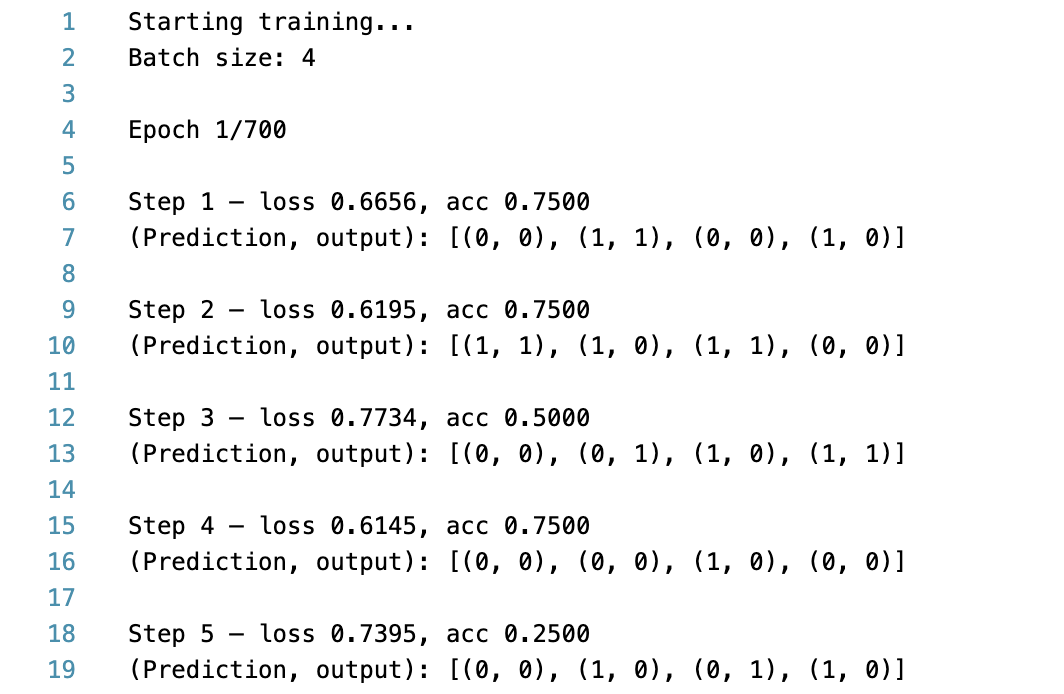
\includegraphics[width=0.5\textwidth]{images/training_log_example.png}
    \caption{Example first few lines from the log file after training}
    \label{fig:training_log_example}
\end{figure}

\begin{figure}[htbp]
    \centering
    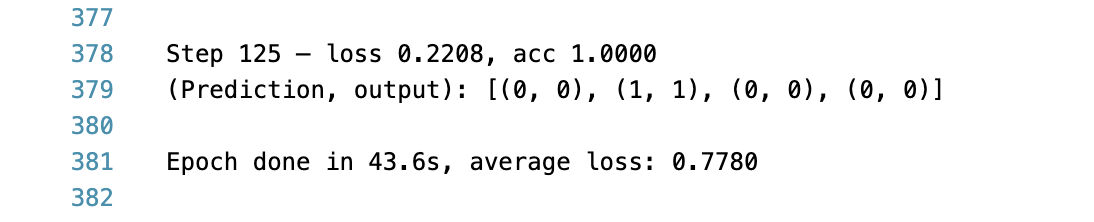
\includegraphics[width=0.5\textwidth]{images/training_log_example2.png}
    \caption{Example of log file at the end of an epoch}
    \label{fig:training_log_example2}
\end{figure}
\bigskip

The batch size was set as four through trial and error on the Boston College High Performance Computer. Four data points per batch allowed for the GPU to perform the training without exceeding the GPU's memory. The following steps per epoch and epochs were calculated to cover as much of the data as a result of the batch size being restricted to four. Finally, after logging, the model will repeat this loop until all epochs are completed and then save out the model to a folder.

\subsection{Testing The Trained Model}

After the training script saves out the model, it is loaded into the test script. This script loads the data in a similar process as the training script. Then, each batch is feed through the model. The data point's true values are appended to an array with their corresponding predictions being appended to a separate array. These arrays are compared to ensure that the model has been feed all the entries. Then, using the sklearn library, the following metrics are calculated and outputted to a log file:

\begin{itemize}
\item Accuracy Score
\item Precision Score
\item Recall Score
\item F1 Score
\end{itemize}

\section{Model Evaluation}

The model was trained on two data sets -- the combined data set and the Prime-Vul data set. Table~\ref{tab:metrics} summarizes the overall classification metrics for each model.

\begin{table}[ht]
  \centering
  \begin{tabular}{|l|c|c|}
    \hline
    \textbf{Metric}   & \textbf{Combined Data Set Model} & \textbf{Prime-Vul Data Set Model} \\ 
    \hline 
    Accuracy          & 88.48\%                          & 77.74\%                  \\ 
    \hline
    Precision         & 32.96\%                          & 32.16\%                  \\ 
    \hline
    Recall            & 95.49\%                          & 76.11\%                  \\ 
    \hline
    F1 Score          & 49.01\%                          & 45.21\%                  \\ 
    \hline
  \end{tabular}
  \caption{Overall performance metrics on the two evaluation datasets.}
  \label{tab:metrics}
\end{table}

\pagebreak

The Combined Data Set model achieves a high accuracy of 88.48 \%, driven largely by its ability to correctly identify the majority class (non-vulnerable functions). Its recall of 95.49 \% indicates that it successfully captures almost all true vulnerable cases; however, at the expense of precision (32.96 \%), leading to a moderate F1 Score of 49.01 \%.  

In contrast, the Prime-Vul Data Set model shows lower overall accuracy (77.74 \%) and recall (76.11 \%), reflecting the increased difficulty of this focused subset. Its precision remains similar (32.16 \%), yielding an F1 Score of 45.21 \%. This suggests that while the model generalizes well across the full dataset, its performance degrades somewhat when restricted to the prime-vulnerability domain.

To better understand where each model makes errors, we examine the confusion matrices below. Table~\ref{tab:confmat-large} shows the Combined Data Set results on 27,900 examples, and Table~\ref{tab:confmat-small} shows the Prime-Vul Data Set results on 7,456 examples.


\begin{table}[ht]
  \centering
  \begin{tabular}{c|cc}
    & \textbf{Pred = 0} & \textbf{Pred = 1} \\ \hline
  \textbf{Actual = 0} & 23,141 & 3,141 \\
  \textbf{Actual = 1} &    74  & 1,544 \\
  \end{tabular}
  \caption{Confusion matrix for the Combined Data Set model (27,900 examples).}
  \label{tab:confmat-large}
\end{table}

In the Combined Data Set confusion matrix, the model correctly labels 23,141 of 26,282 non-vulnerable samples (true negatives) and 1,544 of 1,618 vulnerable samples (true positives). Only 74 vulnerable samples are missed (false negatives), confirming the high recall. However, 3,141 non-vulnerable samples are incorrectly flagged as vulnerable (false positives), which drives down the precision.

\begin{table}[ht]
  \centering
  \begin{tabular}{c|cc}
    & \textbf{Pred = 0} & \textbf{Pred = 1} \\ \hline
  \textbf{Actual = 0} & 5,112 & 1,444 \\
  \textbf{Actual = 1} &  215  &   685 \\
  \end{tabular}
  \caption{Confusion matrix for the Prime-Vul Data Set model (7,456 examples).}
  \label{tab:confmat-small}
\end{table}

On the Prime-Vul Data Set, the model still identifies the majority of non-vulnerable samples correctly (5,112 true negatives), but it misses more vulnerable cases (215 false negatives) relative to the smaller positive class (900 samples). The increase in both false positives (1,444) and false negatives reflects the greater challenge of this domain and explains the drop in both accuracy and recall.

Overall, these results highlight the trade-off between capturing as many true vulnerabilities as possible (recall) and avoiding excessive false alarms (precision). Tuning this balance will depend on the practical needs of the security pipeline: whether catching every possible vulnerability is paramount or reducing investigator workload from false positives is more critical.

\newpage

\section{Contribution Timeline}
\textbf{01/22: Alex, Sara, Drew, Bryan} First team meeting where project ideas were
brainstormed. Google doc was created to store ideas and research \\
\textbf{01/23: Drew, Bryan} Team meeting with Prof. Bento to discuss project ideas.
Code Vulnerability project was chosen \\
\textbf{01/27: Alex, Sara, Drew, Bryan} Team meeting to discuss strategy, proficiencies, 
and research approach \\
\textbf{01/29: Alex} Research on VulKG knowledge-graph. Wrote the abstract. \\
\textbf{01/30: Drew} Research on DiverseVul database. Wrote behaviours section \\
\textbf{01/30: Sara} Research to find papers and literature related to the topic \\
\textbf{01/31: Alex, Drew} Meeting with Professor Bento, discussing progress and databases \\
\textbf{01/31: Sara} Research to find so Python databases \\
\textbf{01/31: Alex} Research on the PrimeVul database and wrote about it. \\
\textbf{02/01: Bryan} Research on current machine learning cybersecurity issues. Wrote
introduction. Found and wrote up a summary about the OSV database \\
\textbf{02/01: Drew} Wrote the Related Works section \\
\textbf{02/02: Drew} Created code to run the functions on ChatGPT and record the loss \\
\textbf{02/03: Alex} Created code to graph data from ChatGPT vulnerability detection loss \\
\textbf{02/05: Alex} Tested "blind guesses" data on first 1000 entries in train dataset \\
\textbf{02/07: Alex, Drew, Bryan, Sara} Researched the NVD API, and tried to get it to run faster \\
\textbf{02/08: Drew} Researched fine-tuning of existing models for improved accuracy \\
\textbf{02/15: Alex} Researched Vul-LMGNN, a pre-existing model using GNN architecture \\
\textbf{02/16: Alex} Researched pre-existing models, including CodeT5 and CodeBERT for fine-tuning \\
\textbf{02/16: Bryan} Experimented with batch and parallelizing the API script \\
\textbf{02/17: Alex} Attempted to fine-tune CodeBERT on first 1000 entries of dataset \\
\textbf{02/18: Drew} Decreased the load time of CVSS scores from hours to minutes through a web scraping algorithm instead of an API call \\
\textbf{02/25: Alex, Drew, Bryan, Sara} Scraped 44,000 entries each in the train dataset to get their CVSS 2.0 vulnerability score and put into reformatted dataset \\
\textbf{02/26: Alex} Scraped for validation dataset \\
\textbf{02/26: Bryan} Began implementing codeT5 and troubleshooting \\
\textbf{03/08: Drew} Created an algorithm to format data for mistral fine-tuning \\
\textbf{03/09: Drew} Ran fine tuning on Mistral through a python script (failure) \\
\textbf{03/10: Alex} Scraped for test dataset \\
\textbf{03/13: Alex, Drew, Bryan, Sara} Met to discuss architecture, discovered GNNs \\
\textbf{03/17: Alex, Drew} Researched CPGs \\
\textbf{03/18: Alex} Read paper on ANGEL model \\
\textbf{03/19: Drew} Created an algorithm to create graphs from code snippets and functions \\
\textbf{03/19: Bryan} Read and wrote about the general transformer architecture \\
\textbf{03/19: Sara} Research on cost of data breach in the past years and how these have been handled \\
\textbf{03/19: Drew} Research on GNNs \\
\textbf{03/20: Sara} Read other articles about problems of ML in the computer security field \\
\textbf{03/20: Alex} Updated datasets in github to contain "func\_hash", file\_info.json, and file\_contents zip \\
\textbf{03/20: Alex} Wrote up sections on Flawfinder, ANGEL \\
\textbf{03/20: Alex} Researched AMPLE GNN model \\
\textbf{03/20: Bryan} Further implementing codeT5 and test train speeds and losses \\
\textbf{03/20: Drew} Wrote the experimentation section of the LaTeX \\
\textbf{03/21: Sara} Researched more about the mechanisms behind the pitfalls \\
\textbf{03/21: Sara} Analyzed how much the databases have been used by the research community (paperswithcode website) \\
\textbf{03/21: Alex} Wrote about AMPLE model \\

\nocite{*}
\bibliographystyle{plain}  % Changed to IEEE style for numbered references
\bibliography{bibliography}

\end{document}